\def\i{\item}
\graphicspath{{../pictures/vande29/}}
\chapter{Chương 5}
\section{Độ dài đoạn thẳng. Trung điểm đoạn thẳng}
\subsection{Kiến thức} 
\subsubsection{Độ dài đoạn thẳng} 
\begin{enumerate}[--, leftmargin=*]
	\i Mỗi đoạn thẳng có một độ dài. Khi chọn một đơn vị độ dài thì độ dài mỗi đoạn thẳng được biểu diễn bởi một số dương (thường viết kèm đơn vị).
	\i Độ dài đoạn thẳng $AB$ còn gọi là khoảng cách giữa hai điểm $A$ và $B$. Ta quy ước khoảng cách giữa hai điểm trùng nhau bằng 0 (đơn vị).
	\i Nếu điểm $B$ nằm giữa điểm $A$ và $C$ thì $AB+BC=AC$.
	\begin{center}
		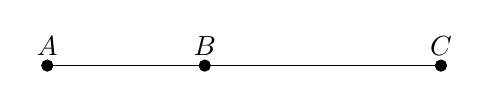
\begin{tikzpicture}
			\draw (0,0) -- (5,0);
			\filldraw[black] (0,0) circle[radius = 2pt] node [above] {$A$};
			\filldraw[black] (2,0) circle[radius = 2pt] node [above] {$B$};
			\filldraw[black] (5,0) circle[radius = 2pt] node [above] {$C$};
		\end{tikzpicture}
	\end{center}
\end{enumerate}
\subsubsection{So sánh độ dài hai đoạn thẳng}
\begin{enumerate}[--, leftmargin=*]
	\i Hai đoạn thẳng $AB$ và $EG$có cùng độ dài. Ta viết $AB=EG$ và nói đoạn thẳng $AB$ bằng đoạn thẳng $EG$.
	\i Đoạn thẳng $AB<CD$ và nói $AB$ ngắn hơn $CD$; hoặc $CD>AB$ và nói $CD$ dài hơn $AB$.
\end{enumerate}
\subsubsection{Trung điểm của đoạn thẳng}
\begin{enumerate}[--, leftmargin=*]
	\i Trung điểm $M$ của đoạn thẳng $AB$ là điểm nằm giữa $A,B$ sao cho $MA=MB$. Khi đó ta có: $MA=MB=\dfrac{AB}{2}$.
\end{enumerate}
\subsection{Thực hành giải toán}
\begin{vd}
	\begin{enumerate}[a), leftmargin=*]
		\i Vẽ đoạn thẳng $AB=4cm$. Vẽ $I$ là trung điểm của $AB$.
		\i Vẽ $C$ sao cho $IC=1cm$.
	\end{enumerate}
	\loigiai{
		\begin{enumerate}[a), leftmargin=*]
			\i 
\begin{tikzpicture}
				\draw (0,0) -- (5,0);
				\filldraw[black] (0,0) circle[radius = 2pt] node [above] {$A$};
				\filldraw[black] (2,0) circle[radius = 2pt] node [above] {$I$};
				\filldraw[black] (4,0) circle[radius = 2pt] node [above] {$B$};
			\end{tikzpicture}
			\i TH1: $C$ nằm giữa $A$ và $I$\\
			
\begin{tikzpicture}
				\draw (0,0) -- (5,0);
				\filldraw[black] (0,0) circle[radius = 2pt] node [above] {$A$};
				\filldraw[black] (1,0) circle[radius = 2pt] node [above] {$C$};
				\filldraw[black] (2,0) circle[radius = 2pt] node [above] {$I$};
				\filldraw[black] (4,0) circle[radius = 2pt] node [above] {$B$};
			\end{tikzpicture}\\
			TH2: $I$ nằm giữa $A$ và $C$\\
			
\begin{tikzpicture}
				\draw (0,0) -- (5,0);
				\filldraw[black] (0,0) circle[radius = 2pt] node [above] {$A$};
				\filldraw[black] (2,0) circle[radius = 2pt] node [above] {$I$};
				\filldraw[black] (3,0) circle[radius = 2pt] node [above] {$C$};
				\filldraw[black] (4,0) circle[radius = 2pt] node [above] {$B$};
			\end{tikzpicture}
	\end{enumerate}}
\end{vd}
\begin{vd}
	Vẽ tia $Ox$, trên $Ox$ lấy $A,B$sao cho $OA=2cm;OB=5cm$.
	\begin{enumerate}[a), leftmargin=*]
		\i Tính $AB$.
		\i Trên tia đối của $Ox$ vẽ điểm $C$ sao cho $OC=2cm$. Hỏi $O$ có phải là trung điểm của $CA$ không? Vì sao? Tính $CA$.
	\end{enumerate}
	\loigiai{
		\begin{enumerate}[a), leftmargin=*]
			\i Vì $A$ nằm giữa $O,B$ nên $OA+AB=OB$\\
			$\Rightarrow 2+AB=5$ \\ 
			$\Rightarrow AB=5-2$ \\ 
			$\Rightarrow AB=3$ \\ 
			\begin{center}
				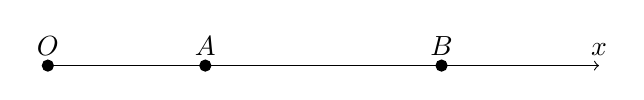
\begin{tikzpicture}
					\draw[->] (0,0) -- (7,0);
					\filldraw[black] (0,0) circle[radius = 2pt] node [above] {$O$};
					\filldraw[black] (2,0) circle[radius = 2pt] node [above] {$A$};
					\draw[black] (7,0) node [above] {$x$};
					\filldraw[black] (5,0) circle[radius = 2pt] node [above] {$B$};
				\end{tikzpicture}
			\end{center}
			\i $O$ là trung điểm của $CA$ vì $O$ nằm giữa $C,A$ và $OC=OA=2cm$.\\
			Ta có: $O$ là trung điểm của $CA$ nên: $CA=2OA=2.2=4cm$
	\end{enumerate}}
\end{vd}
\begin{vd}
	Cho đoạn thẳng $AB=8cm$. Gọi $I$ là trung điểm của $AB$.
	\begin{enumerate}[a), leftmargin=*]
		\i Tính độ dài $AI$.
		\i Trên $AB$ lấy hai điểm $C,D$ sao cho $AC=1cm;BD=1cm$. Chứng tỏ $I$ là trung điểm của $CD$.
	\end{enumerate}
	\loigiai{
		\begin{enumerate}[a), leftmargin=*]
			\i Vì $I$ là trung điểm của $AB$ nên $AI=BI=\dfrac{AB}{2}=\dfrac{8}{2}=4$ (cm).\\
			Vậy $AI=4cm$.
			\i Vì $C$ nằm giữa $A,I$ nên $AC+CI=AI\Rightarrow 1+CI=4\Rightarrow CI=3$ (cm)\\
			Vì $D$ nằm giữa $I,B$ nên $ID+DB=BI\Rightarrow DI+1=4\Rightarrow DI=4-1=3$ (cm)\\
			$\Rightarrow CI=ID$\\
			Vì $I$ nằm giữa $B,C$ và $CI=BI$ nên $I$ là trung điểm $BC$.
	\end{enumerate}}
\end{vd}
\subsection{Bài tập tự luyện}
\Opensolutionfile{loigiaichung}[loigiaichuong29]
\subsubsection*{Mức độ cơ bản}
\begin{bt}
	Vẽ đoạn thẳng $AC$ có độ dài $5cm$. Xác định trung điểm $I$ của đoạn thẳng đó.
	\begin{loigiaichuong29}
		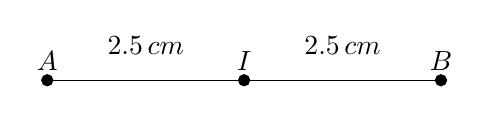
\begin{tikzpicture}
			\draw (0,0) --(5,0);
			\filldraw[black] (0,0) circle[radius = 2pt] node [above] {$A$};
			\filldraw[black] (2.5,0) circle[radius = 2pt] node [above] {$I$};
			\filldraw[black] (5,0) circle[radius = 2pt] node [above] {$B$};
			
			\draw (1.25,0.2) node [above] {$2.5\, cm$};
			\draw (3.75,0.2) node [above] {$2.5\, cm$};
		\end{tikzpicture}
	\end{loigiaichuong29}
\end{bt}
\begin{bt}
	Cho các đoạn thẳng dưới đây:
	\begin{center}
		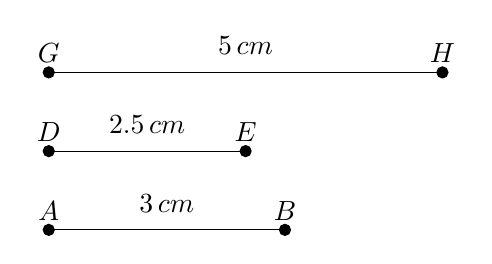
\begin{tikzpicture}
			\draw (0,0) -- (3, 0) (0,1) -- (2.5, 1) (0,2) -- (5,2);
			\filldraw[black] (0,0) circle[radius = 2pt] node[above]{$A$};
			\filldraw[black] (3,0) circle[radius = 2pt] node[above]{$B$};
			\filldraw[black] (0,1) circle[radius = 2pt] node[above]{$D$};
			\filldraw[black] (2.5,1) circle[radius = 2pt] node[above]{$E$};
			\filldraw[black] (0,2) circle[radius = 2pt] node[above]{$G$};
			\filldraw[black] (5,2) circle[radius = 2pt] node[above]{$H$};
			
			\draw (1.5,0.1) node[above]{$3\,cm$};
			\draw (1.25,1.1) node[above]{$2.5\,cm$};
			\draw (2.5,2.1) node[above]{$5\,cm$};
		\end{tikzpicture}
	\end{center}
	Em hãy vẽ tiếp mỗi hình sao cho $I$ là trung điểm của $AB$, $E$ là trung điểm của $DF$ và $G$ là trung điểm của $HK$.
	\begin{loigiaichuong29}
		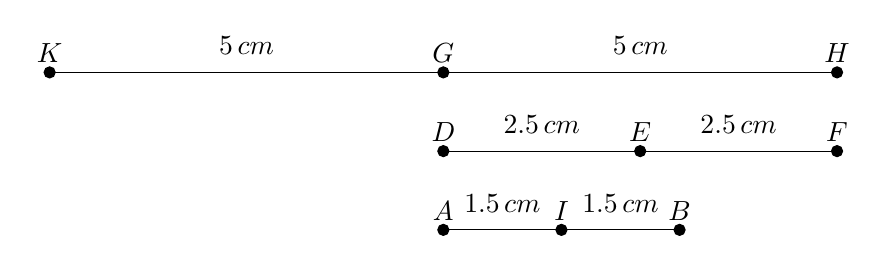
\begin{tikzpicture}
			\draw (0,0) -- (3, 0) (0,1) -- (2.5, 1) -- (5,1) (0,2) -- (5,2) (0,2) -- (-5,2);
			\filldraw[black] (0,0) circle[radius = 2pt] node[above]{$A$};
			\filldraw[black] (3,0) circle[radius = 2pt] node[above]{$B$};
			\filldraw[black] (1.5,0) circle[radius = 2pt] node[above]{$I$};
			\filldraw[black] (0,1) circle[radius = 2pt] node[above]{$D$};
			\filldraw[black] (2.5,1) circle[radius = 2pt] node[above]{$E$};
			\filldraw[black] (5,1) circle[radius = 2pt] node[above]{$F$};
			\filldraw[black] (0,2) circle[radius = 2pt] node[above]{$G$};
			\filldraw[black] (5,2) circle[radius = 2pt] node[above]{$H$};
			\filldraw[black] (-5,2) circle[radius = 2pt] node[above]{$K$};
			
			\draw (0.75,0.1) node[above]{$1.5\,cm$};
			\draw (2.25,0.1) node[above]{$1.5\,cm$};
			\draw (1.25,1.1) node[above]{$2.5\,cm$};
			\draw (3.75,1.1) node[above]{$2.5\,cm$};
			\draw (2.5,2.1) node[above]{$5\,cm$};
			\draw (-2.5,2.1)node[above]{$5\,cm$};
		\end{tikzpicture}
	\end{loigiaichuong29}
\end{bt}
\begin{bt}
	Cho đoạn thẳng $AB=5cm$. Trên tia $BA$ lấy điểm $C$ sao cho $BC=3cm$. Trên tia đối của tia $BA$ lấy điểm $D$ sao cho $BD=1cm$. Tính các độ dài $AD$ và $AC$.
	\begin{loigiaichuong29}
		Vì  $C$ nằm giữa $A,B$ nên ta có: $AB=AC+BC$
		
		$\Rightarrow 5=AC+3\Rightarrow AC=5-3=2$ (cm)
		
		Vì $B$ nằm giữa $A,D$ nên $AD=AB+BD$
		
		$\Rightarrow AD=5+1=6$ (cm)
	\end{loigiaichuong29}
\end{bt}
\begin{bt}
	\begin{enumerate}[a), leftmargin=*]
		\i Trên tia $Ox$ lấy điểm $A$ sao cho $OA=5cm$ và điểm $B$ sao cho $AB=9cm$. Tính $OB$.
		\i Trên tia $Ax$ lấy $M,N$ sao cho $AM=7cm,MN=2cm$. Tính $AN$.
	\end{enumerate}
	\begin{loigiaichuong29}
		\begin{enumerate}[a),leftmargin=*]
			\i	Vì $A$ nằm giữa $O,B$ nên $OB=OA+AB=5+9=14\left( cm \right)$
			\begin{center}
				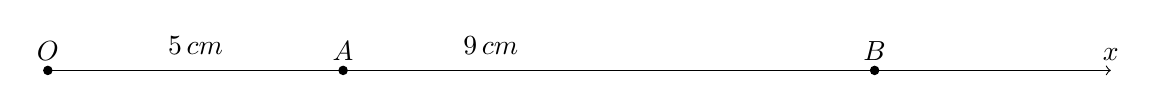
\begin{tikzpicture}[scale=0.75]
					\draw[->] (0,0) -- (18,0);
					\filldraw[black] (0,0) circle[radius = 2pt] node [above] {$O$};
					\filldraw[black] (5,0) circle[radius = 2pt] node [above] {$A$};
					\filldraw[black] (14,0) circle[radius = 2pt] node [above] {$B$};
					\draw (18,0) node[above] {$x$};		
					\draw (2.5,0.1) node[above] {$5\,cm$};		
					\draw (7.5,0.1) node[above] {$9\,cm$};						
				\end{tikzpicture}
			\end{center}
			\i TH1: $M$ nằm giữa $A,N$\\
			Ta có: $AN=AM+MN=7+2=9$ (cm)
			\begin{center}
				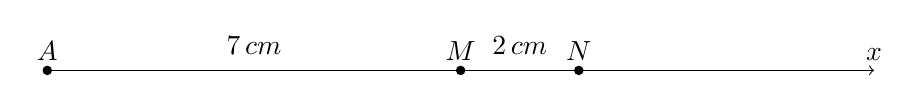
\begin{tikzpicture}[scale=0.75]
					\draw[->] (0,0) -- (14,0);
					\filldraw[black] (0,0) circle[radius = 2pt] node [above] {$A$};
					\filldraw[black] (7,0) circle[radius = 2pt] node [above] {$M$};
					\filldraw[black] (9,0) circle[radius = 2pt] node [above] {$N$};
					\draw (14,0) node[above] {$x$};		
					\draw (3.5,0.1) node[above] {$7\,cm$};		
					\draw (8,0.1) node[above] {$2\,cm$};						
				\end{tikzpicture}
			\end{center}
			TH2: $N$ nằm giữa $A,M$\\
			Ta có: $AM=AN+NM$\\
			$\Rightarrow 7 = AN + 2$\\
			$\Rightarrow AN = 7 - 2 = 5$ (cm).
		\end{enumerate}
	\end{loigiaichuong29}
\end{bt}
\begin{bt}
	Cho đoạn thẳng $AB=10cm$, điểm $M$ thuộc $AB$. Tính độ dài $MA,MB$ biết $MB-MA=4cm$.
	\begin{loigiaichuong29}
		Vì $M$ thuộc đoạn thẳng $AB$  nên ta có: $AB = MB + MA$\\
		$\Rightarrow 10 = MB + MA$\\
		Mà $MB - MA = 4$\\
		Khi đó $MB = 7$ cm; $MA = 3$ cm.
	\end{loigiaichuong29}
\end{bt}
\begin{bt}
	Cho hình vẽ sau. Biết $I$ là trung điểm của$MN$, $P$ là trung điểm của $MI$. Biết rằng $PI=3cm$. Hãy tính độ dài đoạn thẳng $MN$.
	\begin{center}
		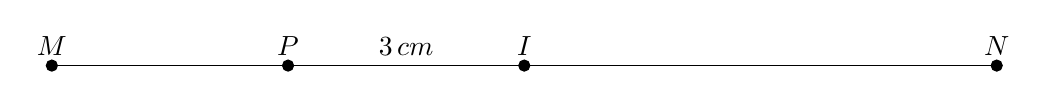
\begin{tikzpicture}
			\draw (0,0) -- (12, 0);
			\filldraw[black] (0,0) circle[radius = 2pt] node [above] {$M$};
			\filldraw[black] (3,0) circle[radius = 2pt] node [above] {$P$};
			\filldraw[black] (6,0) circle[radius = 2pt] node [above] {$I$};
			\filldraw[black] (12,0) circle[radius = 2pt] node [above] {$N$};
			\draw (4.5,0) node[above] {$3\, cm$};		
		\end{tikzpicture}
	\end{center}
	\begin{loigiaichuong29}
		Vì $P$ là trung điểm của $MI$ nên ta có: $MP = IP = \dfrac{MI}{2}$\\
		$\Rightarrow MI = 2IP = 2\cdot 3 = 6$ (cm)\\
		Vì $I$ là trung điểm của $MN$ nên ta có: $MI = IN = \dfrac{MN}{2}$\\
		$\Rightarrow MN = 2MI = 2\cdot 6 = 12$ (cm)\\
		Vậy $MN = 12$ (cm)
	\end{loigiaichuong29}
\end{bt}
\begin{bt}
	Giả sử em muốn tìm điểm chính giữa của chiều dài bàn học. Em sẽ làm như thế nào nếu:
	\begin{enumerate}[a), leftmargin=*]
		\i Dùng thước đo độ dài.
		\i Chỉ dùng một sợi dây đủ dài.
	\end{enumerate}
	\begin{loigiaichuong29}
		\begin{enumerate}[a),leftmargin=*]
			\i Khi sử dụng thước đo độ dài:
			\begin{enumerate}[+,leftmargin=*]
				\i Đo độ dài của bàn học và ghi chú lại số liệu
				\i Điểm chính giữa của bàn học chính là trung điểm của đoạn thẳng đo được
				\i Dựa vào số liệu đã ghi chú và áp dụng công thức tính trung điểm đoạn thẳng xác định số đo
				\i Sử dụng số đo tính toán được áp dụng lên bàn học đó là điểm chính giữa của bàn
			\end{enumerate}
			\i Khi sử dụng đoạn dây vừa đủ:
			\begin{enumerate}[+,leftmargin=*]
				\i Điểm chính giữa của bàn học là trung điểm của đoạn dây chúng ta sử dụng
				\i Gấp đôi đoạn dây lại sao cho hai đầu dây bằng nhau, đánh dấu điểm chính giữa của đoạn dây
				\i Khi đó điểm đánh dấu chính là trung điểm của đoạn dây hay cũng là điểm chính giữa của bàn học
			\end{enumerate}
		\end{enumerate}
	\end{loigiaichuong29}
\end{bt}
\begin{bt}
	Vòng quay mặt trời của một khu vui chơi có điểm thấp nhất là $8m$(so với mặt đất) và điểm cao nhất là $64m$. Hỏi trục của vòng quay nằm ở độ cao nào so với mặt đất? (Tìm hình vẽ minh hoạ)
	\begin{loigiaichuong29}
		Chọn điểm $A$  trùng với điểm thấp nhất của vòng quay mặt trời (so với mặt đất)
		
		Chọn điểm $B$  trùng với điểm cao nhất của vòng quay mặt trời (so với mặt đất)
		
		Khi đó, độ đài đoạn thẳng  $AB$ là: $AB = 64-8 = 56$ (cm)
		
		Theo cách xây dựng của vòng quay mặt trời thì điểm cao nhất của trục sẽ trùng với trung điểm của đoạn thẳng  $AB$, nên trung điểm của đoạn thẳng $AB$ nằm ở độ cao là: $\dfrac{AB}{2} = \dfrac{56}{2} = 28$ (m) 
		Như vậy, trục của vòng quay mặt trời sẽ nằm ở độ cao $28 + 8 = 36$ (m) 
	\end{loigiaichuong29}
\end{bt}
\begin{bt}
	Cho điểm $O$ thuộc đường thẳng $xy$. Điểm $M$ thuộc tia $Ox$, điểm $N$ thuộc tia $Oy$ sao cho $OM=3cm$, $ON=6cm$. Gọi $P$ là trung điểm của $ON$. Chứng tỏ rằng $O$ là trung điểm của $PM$.
	\begin{loigiaichuong29}
		Vì $P$ là trung điểm của $ON$ nên ta có: $OP = PN = \dfrac{ON}{2} = \dfrac{6}{2} = 3$ (cm)
		
		Vì $O$ nằm giữa $M,P$ và $OM=OP=3cm$ nên $O$ là trung điểm của $MP$.
	\end{loigiaichuong29}
	\begin{center}
		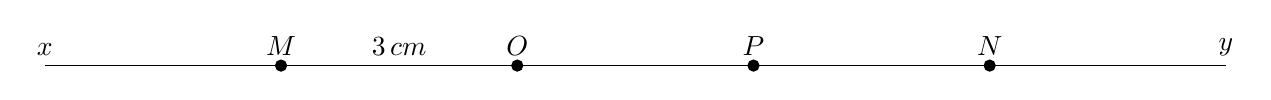
\begin{tikzpicture}
			\draw (0,0) -- (15, 0);
			\filldraw[black] (3,0) circle[radius = 2pt] node [above] {$M$};
			\filldraw[black] (6,0) circle[radius = 2pt] node [above] {$O$};
			\filldraw[black] (9,0) circle[radius = 2pt] node [above] {$P$};
			\filldraw[black] (12,0) circle[radius = 2pt] node [above] {$N$};
			\draw (4.5,0) node[above] {$3\, cm$};
			\draw (0,0) node[above] {$x$};	
			\draw (15,0) node[above] {$y$};
		\end{tikzpicture}
	\end{center}
\end{bt}
\begin{bt}
	Cho đoạn thẳng $AB$ có độ dài là $a$. Trên tia $AB$ lấy điểm $M$ sao cho $AM=\dfrac{a}{2}$. Chứng tỏ rằng điểm $M$ là trung điểm của $AB$.
	\begin{loigiaichuong29}
		Vì $M$ nằm giữa $A,B$ và $AM=MB=\dfrac{AB}{2}=\dfrac{a}{2}$ nên $M$ là trung điểm của đoạn thẳng$AB$
		\begin{center}
			\begin{tikzpicture}
				\draw (0,0) -- (8,0);
				\filldraw[black] (0,0) circle[radius = 2pt] node [above] {$A$};
				\filldraw[black] (3,0) circle[radius = 2pt] node [above] {$M$};
				\filldraw[black] (6,0) circle[radius = 2pt] node [above] {$B$};
				\draw (1.5,0.1) node[above] {$\dfrac{a}{2}$};	
			\end{tikzpicture}
		\end{center}
	\end{loigiaichuong29}
\end{bt}
\subsubsection*{Mức độ nâng cao}
\begin{bt}
	Cho đoạn thẳng $AB$, trên đoạn thẳng $AB$ lấy hai điểm $C,D$ sao cho $AC=BD$. Chứng tỏ rằng $AD=BC$.
	\begin{loigiaichuong29}
		TH1: 
		\begin{center}
			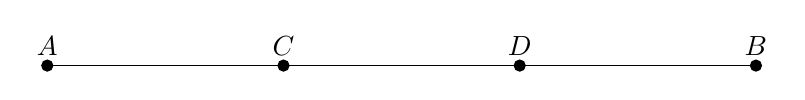
\begin{tikzpicture}
				\draw (0,0) -- (9,0);
				\filldraw[black] (0,0) circle[radius = 2pt] node [above] {$A$};
				\filldraw[black] (3,0) circle[radius = 2pt] node [above] {$C$};
				\filldraw[black] (6,0) circle[radius = 2pt] node [above] {$D$};
				\filldraw[black] (9,0) circle[radius = 2pt] node [above] {$B$};
			\end{tikzpicture}
		\end{center}
		Vì $C$ nằm giữa $A,D$ nên ta có: $AC+CD=AD$\\
		Vì $D$ nằm giữa $B,C$ nên ta có: $BC+CD=BC$\\
		Mà $AC=BD$ và $CD$ chung $\Rightarrow AD=BC$\\
		TH2:
		\begin{center}
			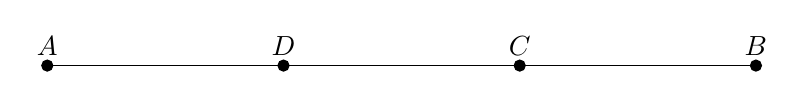
\begin{tikzpicture}
				\draw (0,0) -- (9,0);
				\filldraw[black] (0,0) circle[radius = 2pt] node [above] {$A$};
				\filldraw[black] (3,0) circle[radius = 2pt] node [above] {$D$};
				\filldraw[black] (6,0) circle[radius = 2pt] node [above] {$C$};
				\filldraw[black] (9,0) circle[radius = 2pt] node [above] {$B$};
			\end{tikzpicture}
		\end{center}
		Vì $D$ nằm giữa $A,C$ nên ta có: $AC=AD+DC\Rightarrow AD=AC-DC$\\
		Vì $C$ nằm giữa $B,D$ nên ta có: $BD=BC+DC\Rightarrow BC=BD-DC$\\
		Mà $AC=BD$ và $DC$ chung $\Rightarrow AD=BC$
	\end{loigiaichuong29}
\end{bt}
\begin{bt}
	Cho hai điểm $A,B$ thuộc tia $Oz$ sao cho $OA=a$, $AB=b\left( b>a \right)$. Gọi $C$ là trung điểm của đoạn thẳng $OB$. Tìm độ dài đoạn thẳng $AC$?
	\begin{loigiaichuong29}
		Vì $A$ nằm giữa $O,B$ nên ta có: $OB=OA+AB=a+b$\\
		Vì $C$ là trung điểm của $OB$ nên ta có: $OC=CB=\dfrac{OB}{2}=\dfrac{a+b}{2}$\\
		Vì $A$ nằm giữa $O,C$ nên ta có: $OC=OA+AC$\\
		\begin{center}
			\begin{tikzpicture}
				\draw (0,0) -- (13,0);
				\filldraw[black] (0,0) circle[radius = 2pt] node [above] {$O$};
				\filldraw[black] (4,0) circle[radius = 2pt] node [above] {$A$};
				\filldraw[black] (5,0) circle[radius = 2pt] node [above] {$C$};
				\filldraw[black] (9,0) circle[radius = 2pt] node [above] {$B$};
				\draw (13,0.1) node[above] {$x$};
			\end{tikzpicture}
		\end{center}
		$\Rightarrow \dfrac{a + b}{2} = a + AC$\\
		$\Rightarrow AC = \dfrac{a+b}{2} - a = \dfrac{b-a}{2}$\\
		Vậy $AC = \dfrac{b-a}{2}$
	\end{loigiaichuong29}
\end{bt}
\begin{bt}
	Cho điểm $A$ nằm giữa hai điểm $B$ và $C$. Điểm $I$ là trung điểm của đoạn thẳng $AB$ và $3AB=4AC$. Biết $BI=4\,cm$. Tính độ dài đoạn thẳng $BC$.
	\begin{loigiaichuong29}
		Vì $A$ nằm giữa $B,C$ và $3AB=4AC$ nên ta chia $BC$ thành 7 phần bằng nhau và xác định điểm $A$ như hình vẽ.
		\begin{center}
			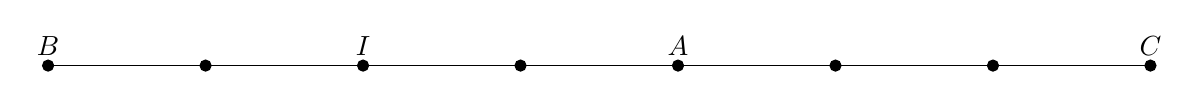
\begin{tikzpicture}
				\draw (0,0) -- (14,0);
				\filldraw[black] (0,0) circle[radius = 2pt] node [above] {$B$};
				\filldraw[black] (2,0) circle[radius = 2pt];
				\filldraw[black] (4,0) circle[radius = 2pt] node [above] {$I$};
				\filldraw[black] (6,0) circle[radius = 2pt];
				\filldraw[black] (8,0) circle[radius = 2pt] node [above] {$A$};
				\filldraw[black] (10,0) circle[radius = 2pt];
				\filldraw[black] (12,0) circle[radius = 2pt];
				\filldraw[black] (14,0) circle[radius = 2pt] node [above] {$C$};
			\end{tikzpicture}
		\end{center}
		Vì $I$ là trung điểm của $AB$ nên ta có: $BI=AI=\dfrac{AB}{2}$\\
		$\Rightarrow AI=2BI=2\cdot4=8$ (cm)\\
		Lại có: $3AB=4AC\Rightarrow AC=\dfrac{3AB}{4}=\dfrac{3\cdot8}{4}=6$ (cm)\\
		Vì $A$ nằm giữa $B,C$ nên ta có: $BC=AB+AC=8+6=14$ (cm)\\
		Vậy $BC=14$ (cm)
	\end{loigiaichuong29}
\end{bt}
\begin{bt}
	Cho đoạn thẳng $AB=1\,cm$. Lấy ${{A}_{1}}$ là trung điểm của đoạn thẳng $AB$, ${{A}_{2}}$ là trung điểm của đoạn thẳng $A{{A}_{1}}$, ${{A}_{3}}$ là trung điểm của đoạn thẳng $A{{A}_{2}}$,\ldots cứ tiếp tục như vậy cho đến ${{A}_{20}}$ là trung điểm của $A{{A}_{19}}$. Tính độ dài $A{{A}_{20}}$.
	\begin{loigiaichuong29}
		Vì ${{A}_{1}}$ là trung điểm của $AB$ nên ta có: $A{{A}_{1}}=AB.\dfrac{1}{2}$ (m)\\
		Vì ${{A}_{2}}$ là trung điểm của $A{{A}_{1}}$ nên ta có: $A{{A}_{2}}=\dfrac{A{{A}_{1}}}{2}=AB\cdot\dfrac{1}{2}\cdot\dfrac{1}{2}$ (m)\\
		Vì ${{A}_{3}}$ là trung điểm của $A{{A}_{2}}$ nên ta có: $A{{A}_{3}}=\dfrac{A{{A}_{2}}}{2}=\dfrac{A{{A}_{1}}}{2}\cdot\dfrac{1}{2}=AB\cdot\dfrac{1}{2}\cdot\dfrac{1}{2}\cdot\dfrac{1}{2}$ (m)\\
		Vì ${{A}_{4}}$ là trung điểm của $A{{A}_{3}}$ nên ta có: $A{{A}_{4}}=\dfrac{A{{A}_{3}}}{2}=\dfrac{A{{A}_{2}}}{2}\cdot\dfrac{1}{2}=\dfrac{A{{A}_{1}}}{2}\cdot\dfrac{1}{2}\cdot\dfrac{1}{2}=AB\cdot\dfrac{1}{2}\cdot\dfrac{1}{2}\cdot\dfrac{1}{2}\cdot\dfrac{1}{2}$ (m)\\
		Như vậy, khi ta lấy trung điểm ${{A}_{n}}$ của $AB$ thì $A{{A}_{n}}=AB\cdot{{ \left(\dfrac{1}{2} \right)}^{n}}$ (m)\\
		Vậy độ dài đoạn thẳng $A{{A}_{20}}=AB.{{\left(\dfrac{1}{2} \right)}^{n}}=1\cdot{{ \left(\dfrac{1}{2} \right)}^{20}}={{\left(\dfrac{1}{2} \right)}^{20}}$ (m)
	\end{loigiaichuong29}
\end{bt}
\begin{bt}
	Cho 10 điểm phân biệt không thẳng hàng vẽ được tất cả bao nhiêu đoạn thẳng có hai đầu mút là 2 trong 10 điểm nói trên?
	\begin{loigiaichuong29}
		Do cứ 2 điểm thì tạo thành 1 đường thẳng và không có 3 điểm nào thẳng hàng nên 10 điểm sẽ nối được với 9 điểm và mỗi đường thẳng sẽ bị trùng nên ta có: 
		
		Số đường thẳng được tạo thành là: $\dfrac{10 \cdot 9}{2}=45 $ (đường thẳng)
		
		Vậy tạo thành được 45 đường thẳng khác nhau có đầu mút là 2 trong 10 điểm đã cho.
	\end{loigiaichuong29}
\end{bt}
\begin{bt}
	Cho biết điểm $M$ nằm giữa 2 điểm $A,B$ .Điểm  $I$ là trung điểm của đoạn thẳng $AB$  và  $5AB=8BM$.  Biết  $MI=2\,cm$ , tính độ dài của đoạn $AB$ 
	\begin{loigiaichuong29}
		Do $5AB = 8BM \Rightarrow Bm = \dfrac{5AB}{8}$\\
		Mà $Bi = \dfrac{AB}{2}$\\
		$\Rightarrow Mi = BM - BI = \dfrac{5}{8}AB - \dfrac{1}{2}AB = \dfrac{1}{8} AB$.\\
		$\Rightarrow \dfrac{1}{8} AB = 2$ (cm)\\
		$\Rightarrow AB = 16$ (cm)
	\end{loigiaichuong29}
	\begin{center}
		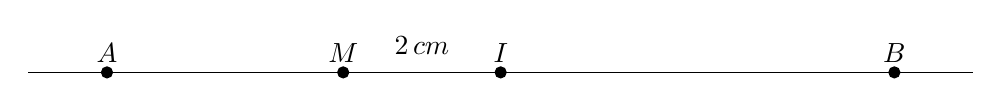
\begin{tikzpicture}
			\draw (0,0) -- (12,0);
			\filldraw[black] (1,0) circle[radius = 2pt] node [above] {$A$};
			\filldraw[black] (4,0) circle[radius = 2pt] node [above] {$M$};
			\filldraw[black] (6,0) circle[radius = 2pt] node [above] {$I$};
			\filldraw[black] (11,0) circle[radius = 2pt] node [above] {$B$};
			\draw (5,0.1) node[above] {$2\, cm$};
		\end{tikzpicture}
	\end{center}
\end{bt}
\begin{bt}
	Cho 2 điểm $A,B$ thuộc tia  $Ox$  sao cho  $OA=a,OB=b\,(b>a)$ 
	$C$ là trung điểm của đoạn $OB.$  Tính độ dài đoạn thẳng  $AB,CA?$ (theo  $a$  và  $b$).
	\begin{loigiaichuong29}
		Vì $OA<OB$ nên $A$ nằm giữa $O$ và $B$ $\Rightarrow AB=b-a$.\\
		Vì $C$ là trung điểm của $OB$ nên $OC=CB=\dfrac{b}{2}$\\
		TH1: Nếu $a<\dfrac{b}{2}$thì $OA<OC\Rightarrow OA+AC=OC\Rightarrow AC=OC-OA=\dfrac{b}{2}-a$\\
		TH2: Nếu $a>\dfrac{b}{2}$thì $OC<OA\Rightarrow OC+AC=OA\Rightarrow AC=OA-OC=a-\dfrac{b}{2}$
		\begin{center}
			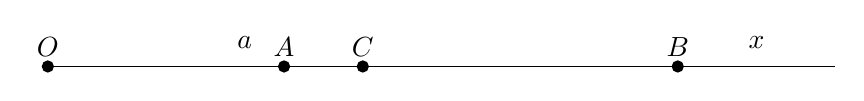
\begin{tikzpicture}
				\draw (0,0) -- (10,0);
				\filldraw[black] (0,0) circle[radius = 2pt] node [above] {$O$};
				\filldraw[black] (3,0) circle[radius = 2pt] node [above] {$A$};
				\filldraw[black] (4,0) circle[radius = 2pt] node [above] {$C$};
				\filldraw[black] (8,0) circle[radius = 2pt] node [above] {$B$};
				\draw (2.5,0.1) node[above] {$a$};
				\draw (9,0.1) node[above] {$x$};
			\end{tikzpicture}
		\end{center}
	\end{loigiaichuong29}
\end{bt}
\begin{bt}
	Cho đường thẳng  $xy$ , điểm  $O$  nằm trên đường thẳng, vẽ 2 điểm  $A,B$ sao cho  $OA=3\,cm$; $OB=8\,cm$.  Trên  $xy$  ta lấy điểm  $C$  sao cho  $OC=a$.  Hãy tìm vị trí của điểm  $C$ và giá trị của  $a$  để  $A$  là trung điểm của  $CB$.
	\begin{loigiaichuong29}
		Ta xét các trường hợp sau:\\
		TH1: $O$ cùng phía với 2 điểm $A,B.$ 
		\begin{center}
			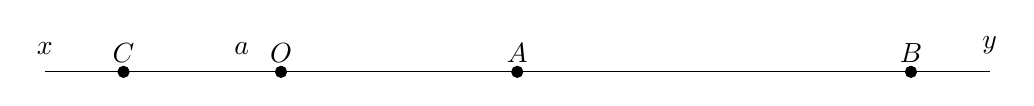
\begin{tikzpicture}
				\draw (0,0) -- (12,0);
				\filldraw[black] (1,0) circle[radius = 2pt] node [above] {$C$};
				\filldraw[black] (3,0) circle[radius = 2pt] node [above] {$O$};
				\filldraw[black] (6,0) circle[radius = 2pt] node [above] {$A$};
				\filldraw[black] (11,0) circle[radius = 2pt] node [above] {$B$};
				\draw (2.5,0.1) node[above] {$a$};
				\draw (0,0.1) node[above] {$x$};
				\draw (12,0.1) node[above] {$y$};
			\end{tikzpicture}
		\end{center}
		Do $OA=3cm$; $OB=8cm$  và $O$ cùng phía với 2 điểm $A,B$  nên $A$  nằm giữa $O$ và $B$.\\
		$\Rightarrow AB=OB-OA=8-3=5$ (cm).\\ 
		$A$  là trung điểm của $CB \Rightarrow C$ thuộc tia đối của tia $AB$  hay $A$  nằm giữa $C,B$ và $AC=AB=5$ (cm).\\
		$\Rightarrow AC>AO \Rightarrow O$  nằm giữa $A,C$.\\
		$\Rightarrow OC=AC-AO=5-3=2$ (cm).\\ 
		TH2: $O$  khác phía với 2 điểm $A,B$.\\ 
		\begin{center}
			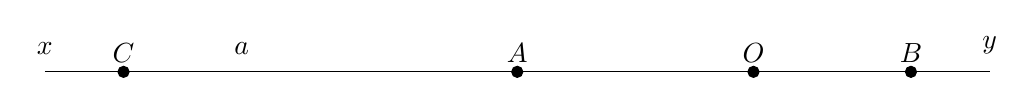
\begin{tikzpicture}
				\draw (0,0) -- (12,0);
				\filldraw[black] (1,0) circle[radius = 2pt] node [above] {$C$};
				\filldraw[black] (9,0) circle[radius = 2pt] node [above] {$O$};
				\filldraw[black] (6,0) circle[radius = 2pt] node [above] {$A$};
				\filldraw[black] (11,0) circle[radius = 2pt] node [above] {$B$};
				\draw (2.5,0.1) node[above] {$a$};
				\draw (0,0.1) node[above] {$x$};
				\draw (12,0.1) node[above] {$y$};
			\end{tikzpicture}
		\end{center}
		Do $O$  khác phía với 2 điểm $A,B$  nên $O$  nằm giữa $A$  và $B$.\\
		$\Rightarrow AB=OA+OB=3+8=11$ (cm).\\ 
		$A$  là trung điểm của $CB \Rightarrow C$ thuộc tia đối của tia $AB$  hay $A$  nằm giữa $C,B$ và $AC=AB=11$ (cm).\\ 
		$\Rightarrow A$ nằm giữa $C,O$ $\Rightarrow OC=OA+AC=3+11=14$ (cm). 
	\end{loigiaichuong29}
\end{bt}
\Closesolutionfile{loigiaichung}






